%=====================================================================
%  DATABASE TECHNOLOGY, MANAGEMENT AND SECURITY
%  Project Report --- Type 4, Experimental / Benchmarking Project
%
%  Built from the course-provided template (db-report-template).
%  Compiler: pdfLaTeX. Bibliography: biber (IEEE style).
%=====================================================================

\documentclass[12pt, a4paper]{article}

%---------------------------------------------------------------------
% Packages
%---------------------------------------------------------------------
\usepackage[a4paper, margin=2.5cm]{geometry}
\usepackage[utf8]{inputenc}
\usepackage[T1]{fontenc}
\usepackage{times}
\usepackage{graphicx}
\usepackage{booktabs}
\usepackage{array}
\usepackage{longtable}
\usepackage{multirow}
\usepackage{amsmath, amssymb}
\usepackage{caption}
\usepackage{subcaption}
\usepackage{enumitem}
\usepackage{setspace}
\usepackage{fancyhdr}
\usepackage{listings}
\usepackage{xcolor}
\usepackage{csquotes}
\usepackage[hidelinks]{hyperref}
\usepackage[nameinlink]{cleveref}

\usepackage[backend=biber, style=ieee, sorting=none]{biblatex}
\addbibresource{references.bib}

%---------------------------------------------------------------------
% Report metadata
%---------------------------------------------------------------------
\newcommand{\CourseName}{Database Technology, Management and Security}
\newcommand{\ReportTitle}{Do Common PostgreSQL Index Tuning Practices Actually Help?}
\newcommand{\ProjectType}{Project Type 4 --- Experimental / Benchmarking Project}
\newcommand{\GroupNumber}{Group XX}
\newcommand{\SubmissionDate}{22 August 2026}
\newcommand{\InstructorName}{Dr.\ Ashraf Uddin}
\newcommand{\InstructorTitle}{Assistant Professor}
\newcommand{\InstructorDept}{Department of Computer Science}
\newcommand{\InstructorInstitution}{American International University-Bangladesh}

%---------------------------------------------------------------------
% Listing style
%---------------------------------------------------------------------
\definecolor{codegray}{gray}{0.95}
\definecolor{codegreen}{rgb}{0,0.5,0}
\definecolor{codeblue}{rgb}{0,0,0.7}
\lstdefinestyle{codestyle}{
    backgroundcolor=\color{codegray},
    basicstyle=\ttfamily\footnotesize,
    keywordstyle=\color{codeblue}\bfseries,
    commentstyle=\color{codegreen}\itshape,
    stringstyle=\color{red!60!black},
    numbers=none,
    frame=single,
    framerule=0pt,
    breaklines=true,
    showstringspaces=false,
    captionpos=b,
    tabsize=2
}
\lstset{style=codestyle}

%---------------------------------------------------------------------
% Headers and footers
%---------------------------------------------------------------------
\pagestyle{fancy}
\fancyhf{}
\fancyhead[L]{\small\CourseName}
\fancyhead[R]{\small\GroupNumber}
\fancyfoot[C]{\thepage}
\renewcommand{\headrulewidth}{0.4pt}

\onehalfspacing

%=====================================================================
\begin{document}

%---------------------------------------------------------------------
% TITLE PAGE
%---------------------------------------------------------------------
\begin{titlepage}
    \centering
    \vspace*{1.5cm}

    {\large \textbf{\CourseName}}\\[0.4cm]
    {\large \ProjectType}\\[2cm]

    \rule{\linewidth}{0.5mm}\\[0.6cm]
    {\LARGE \textbf{\ReportTitle}}\\[0.4cm]
    \rule{\linewidth}{0.5mm}\\[1.8cm]

    {\large \textbf{Submitted By}}\\[0.4cm]
    {\large \textbf{\GroupNumber}}\\[0.5cm]

    \begin{tabular}{@{}ll@{}}
        \toprule
        \textbf{Name} & \textbf{Student ID} \\
        \midrule
        Md. Imtiaj Alam Sajin & 26-94090-2 \\
        \bottomrule
    \end{tabular}\\[1.8cm]

    {\large \textbf{Submitted To}}\\[0.4cm]
    {\large \InstructorName}\\[0.15cm]
    \InstructorTitle\\[0.15cm]
    \InstructorDept\\[0.15cm]
    \InstructorInstitution\\[1cm]

    \vfill
    {\large Submission Date: \SubmissionDate}\\[0.5cm]
\end{titlepage}

%---------------------------------------------------------------------
% DECLARATION OF ORIGINALITY
%---------------------------------------------------------------------
\section*{Declaration of Originality}
\addcontentsline{toc}{section}{Declaration of Originality}
I declare that this report is my own original work. All sources of
information have been acknowledged and cited using the IEEE referencing
style. No part of this report has been copied from any other student's
work or from any other source except where explicitly cited. I
understand that any act of plagiarism will be dealt with according to
the university's academic integrity policy.

All measurements reported here were produced by the software published
with this report~\cite{artifact2026}. Every figure and table is
generated directly from the raw measurement files; no numerical value in
this report was transcribed by hand.

\vspace{1.5cm}
\noindent
\begin{tabular}{@{}p{6cm}@{}}
    \rule{5cm}{0.4pt} \\
    Md. Imtiaj Alam Sajin \\
\end{tabular}

\newpage

%---------------------------------------------------------------------
% ABSTRACT
%---------------------------------------------------------------------
\section*{Abstract}
\addcontentsline{toc}{section}{Abstract}
Choosing the wrong index can make a query orders of magnitude slower,
and a substantial body of practitioner guidance exists to help database
administrators avoid that outcome. This report asks whether that
guidance survives measurement. We built a controlled benchmark that
varies value skew, predicate correlation and physical clustering
independently, and measured 14{,}296 query executions against
PostgreSQL 17.1 across seven table scales, eleven dataset
configurations, ten index configurations and seven cost-model settings.
Ground-truth
cardinality for every predicate is computed from the generated data
rather than taken from the database, so estimation error is measured
directly. The first result is reassuring: with a conventional index
set, PostgreSQL selects a near-optimal access path, erring materially
in only 2.3\% of queries at a median penalty of 1.3\%. The remaining
results are not. Three widely recommended practices are evaluated and
all three are found to backfire under identifiable conditions. Extended
statistics improve cardinality estimates by up to 108 times while
making the affected queries up to 2.7 times slower. Lowering
\texttt{random\_page\_cost} below its default on solid-state storage
makes the workload 2.3 times slower rather than faster. Adding a BRIN
index alongside a B-tree on the same column raises misselection from
2.3\% to 73.3\%, with individual queries degrading by up to 194 times,
while the table is resident in the buffer pool. Measuring five
intermediate scales shows that this last effect does not simply vanish
as the table grows: its frequency collapses once the heap exceeds
\texttt{shared\_buffers}, but its worst case doubles at that same point
and subsides only once queries begin paying physical I/O. Each
behaviour is traced to a specific mechanism visible in the query plan.

\vspace{0.5em}
\noindent\textbf{Keywords:} query optimisation; access path selection;
index selection; cardinality estimation; PostgreSQL; performance
benchmarking

\newpage

%---------------------------------------------------------------------
% FRONT MATTER
%---------------------------------------------------------------------
\tableofcontents
\newpage
\listoffigures
\listoftables
\newpage

%=====================================================================
\section{Introduction}
%=====================================================================

\subsection{Background and Motivation}
A query optimiser's access-path decision, whether to scan a table
sequentially or to use one of several available indexes, is among the
most consequential choices it makes. The problem was formalised in the
System R optimiser~\cite{selinger1979access} and the same cost-based
framework, estimate cardinality then price each candidate path,
underpins PostgreSQL today. The same query can differ by two orders of
magnitude in runtime depending on that single decision.

Because the decision matters and is opaque to the user, a large body of
tuning folklore has grown around it. Administrators are advised to
create extended statistics when columns are
correlated~\cite{pgdocs17createstats}, to lower
\texttt{random\_page\_cost} when running on solid-state
storage~\cite{pgdocs17runtimeconfig}, and to add BRIN indexes on
naturally ordered columns because they are small and cheap to
build~\cite{pgdocs17brin}. This advice appears in official
documentation, vendor engineering blogs and community forums. It is
rarely accompanied by systematic measurement.

\subsection{Problem Statement}
Prior work established that cardinality misestimation is the dominant
source of poor plans~\cite{leis2015good, leis2018query}, but studied
join ordering rather than single-table access-path selection. Whether
the shipped classical planner selects access paths well, and whether
the remedies commonly recommended for it actually improve matters,
has not been examined systematically. This report addresses that gap
through four research questions.

\begin{itemize}[nosep]
    \item \textbf{RQ1.} How often does the PostgreSQL planner select a
      slower access path than one available to it, and what does that
      cost?
    \item \textbf{RQ2.} Which data properties drive misselection: value
      skew, correlation between predicate columns, or physical
      clustering?
    \item \textbf{RQ3.} Is cardinality misestimation the cause, as the
      optimisation literature would predict?
    \item \textbf{RQ4.} Do the three tuning practices named above
      actually improve access-path selection?
\end{itemize}

\subsection{Objectives and Scope}
\begin{itemize}[nosep]
    \item Build a benchmark in which skew, predicate correlation and
      physical clustering vary independently, with exact ground-truth
      cardinality for every predicate.
    \item Quantify PostgreSQL 17's access-path selection quality.
    \item Evaluate three recommended tuning practices empirically and
      explain any failures mechanistically.
    \item Publish a fully reproducible artifact.
\end{itemize}

\noindent
\textbf{Excluded from scope.} Join ordering and join method selection,
which are separate and well-studied problems~\cite{leis2018query};
cold-cache behaviour, because reliably evicting the operating system
page cache is not portable; and multi-user concurrency, since all
measurements are single-session.

\subsection{Report Organization}
\Cref{sec:background} reviews the relevant theory and prior work.
\Cref{sec:methodology} describes the experimental design and
measurement protocol. \Cref{sec:results} presents the results.
\Cref{sec:discussion} interprets them and states threats to validity.
\Cref{sec:conclusion} concludes.

%=====================================================================
\section{Background and Literature Review}
\label{sec:background}
%=====================================================================

\subsection{Key Concepts}

\textbf{Access-path selection.} Given a predicate over a table, the
optimiser enumerates candidate access paths, a sequential scan and one
path per usable index, estimates how many rows each will produce, and
prices each using a cost model~\cite{selinger1979access,
silberschatz2019database}. In PostgreSQL, cost is expressed in
arbitrary units anchored to \texttt{seq\_page\_cost}, with
\texttt{random\_page\_cost} expressing how much more expensive a
randomly fetched page is assumed to be~\cite{pgdocs17indexcost}.

\textbf{Index types.} A B-tree supports equality and range predicates
and returns exact tuple pointers~\cite{graefe2011modern}. A hash index
supports equality only. A BRIN index stores summary information per
block range rather than per tuple, making it very small, but it returns
\emph{candidate block ranges} rather than rows, so matching tuples must
be rechecked. Its usefulness therefore depends entirely on the physical
correlation between indexed value and row position~\cite{pgdocs17brin}.

\textbf{Cardinality estimation.} PostgreSQL estimates the selectivity
of a conjunction by multiplying the per-column selectivities, which
assumes the columns are independent~\cite{pgdocs17planner}. When they
are not, the estimate can be wrong by orders of magnitude. Extended
statistics objects created with \texttt{CREATE STATISTICS} are the
documented remedy~\cite{pgdocs17createstats}.

\subsection{Related Work}

\textbf{Optimiser quality.} Leis et al.~\cite{leis2015good,
leis2018query} showed with the Join Order Benchmark that cardinality
misestimation, not cost-model calibration, dominates plan quality, and
that errors compound multiplicatively through join trees. Their focus
is join ordering; single-table access-path selection is not isolated.
Our results are complementary and, in one respect, opposed: for the
access-path decision we find misestimation is \emph{not} the primary
cause of the misselection observed.

\textbf{Estimation error metrics.}
Moerkotte et al.~\cite{moerkotte2009preventing} introduced q-error, the
symmetric ratio between estimated and actual cardinality, and showed
it bounds plan cost degradation. We adopt it unchanged.

\textbf{Benchmarking methodology.}
Raasveldt et al.~\cite{raasveldt2018fair} catalogue common pitfalls in
database performance testing, including failing to control caching,
reporting single runs, and using measurement instruments whose overhead
depends on the plan being measured. Our protocol in
\Cref{sec:protocol} addresses each of these explicitly.
Wongkham et al.~\cite{wongkham2022updatable} provide a model for
rigorous index benchmarking, in particular the practice of measuring
each index design in isolation rather than inferring its behaviour.

\textbf{System documentation.} The behaviour we report for BRIN is
adjacent to a known difficulty acknowledged on the PostgreSQL hackers
mailing list~\cite{pghackers2019brin}, where BRIN cost estimation is
discussed as unreliable. That discussion concerns the opposite
direction, BRIN being faster but not chosen. We are not aware of a
systematic quantification of the direction reported here.

\subsection{Research Gap}
Three gaps motivate this study. First, access-path selection in the
shipped classical planner has not been isolated and measured in the way
join ordering has. Second, the tuning practices recommended to improve
it are supported by mechanism arguments rather than workload-level
measurement. Third, where effects are reported they are seldom
accompanied by the conditions under which they cease to hold, so
practitioners cannot tell whether a finding applies to them.

%=====================================================================
\section{Methodology}
\label{sec:methodology}
%=====================================================================

\subsection{Overview of Approach}
The study measures, for each query, the execution time of the plan the
planner freely chose against the fastest plan obtainable by restricting
the available indexes. The ratio between them isolates the quality of
the planner's decision from the intrinsic difficulty of the query.

Because PostgreSQL provides no mechanism to hide one index from the
planner while leaving others visible, each candidate access path is
measured by building that index \emph{alone} and running the full query
set. A final configuration builds every index at once, reproducing a
realistic deployment, and is where the planner's actual choice is
observed.

\subsection{Definitions and Metrics}
\label{sec:metrics}

\textbf{q-error}~\cite{moerkotte2009preventing} measures cardinality
misestimation:
\begin{equation}
q(\hat{n}, n) = \frac{\max(\hat{n}, n)}{\min(\hat{n}, n)}
\end{equation}
where $\hat{n}$ is the estimate and $n$ the true row count, both
floored at 1. A value of 1.0 is a perfect estimate. The ratio form is
used because a factor-of-ten underestimate and a factor-of-ten
overestimate are equally damaging to plan choice.

\textbf{Access-path regret} measures the cost of the decision:
\begin{equation}
R(q) = \frac{T_{\text{chosen}}(q)}{\min_{a \in A} T_a(q)}
\end{equation}
where $A$ is the set of index configurations and $T$ is median
execution time. $R = 1$ means the planner made the best available
choice; $R = 4$ means the query took four times longer than necessary.
Because the denominator is the fastest configuration \emph{measured}
rather than a proven optimum, reported regret is a \textbf{lower bound}
on the true penalty.

\textbf{Misselection} is defined as $R > 1.2$. The threshold prevents
run-to-run variation from being counted as a planner error; it is a
judgement call and is stated as such.

\subsection{Data Generation}
Real datasets do not allow one property to be varied while others are
held fixed, so all data is generated. Three factors are controlled
independently, each varied around a uniform, independent baseline so
that every effect is attributable (\Cref{tab:factors}).

\begin{table}[htbp]
    \centering
    \caption{Controlled factors. Eleven dataset configurations result,
    each varying one factor from the baseline.}
    \label{tab:factors}
    \small
    \begin{tabular}{@{}lll@{}}
        \toprule
        \textbf{Factor} & \textbf{Levels} & \textbf{Controls} \\
        \midrule
        \texttt{zipf\_s}        & 0.0, 0.5, 1.0, 1.5 & Value skew of the indexed column \\
        \texttt{dep\_strength}  & 0.0, 0.25, 0.5, 0.75, 1.0 & Strength of the functional dependency $a \rightarrow b$ \\
        \texttt{physical\_corr} & 0.0, 0.5, 0.95, 1.0 & Correlation of value order with row order \\
        \bottomrule
    \end{tabular}
\end{table}

Domain sizes are load-bearing. With one million rows and 100 distinct
values in each of columns $a$ and $b$, an independent conjunction
\texttt{a = va AND b = vb} returns approximately 100 rows, exactly what
the independence assumption predicts. Under a full functional
dependency the same predicate returns all 10{,}000 rows sharing
\texttt{a = va} while the estimate remains at 100. That is a q-error of
100 at one percent selectivity, which is precisely the region where
index and sequential access compete.

All randomness is seeded, so the corpus is byte-for-byte reproducible.

\subsection{Query Families}
Four families are used, each with exactly known true cardinality
computed by counting the generated arrays directly rather than by
asking the database:

\begin{itemize}[nosep]
    \item \textbf{Equality} on the skewed column. Candidate paths:
      hash, B-tree, BRIN, sequential scan.
    \item \textbf{Range} on the skewed column. Hash cannot serve this,
      which tests whether the planner falls back correctly.
    \item \textbf{Range on the physically clustered column.} BRIN's
      most favourable case.
    \item \textbf{Conjunctive} on the correlated pair, in dependent and
      independent variants. The independent variant is the control.
\end{itemize}

\subsection{Measurement Protocol}
\label{sec:protocol}
Every timed execution used
\texttt{EXPLAIN (ANALYZE, BUFFERS, TIMING OFF, FORMAT JSON)}, reading
the top-level \texttt{Execution Time}. Three reasons, each affecting
validity~\cite{raasveldt2018fair}:

\begin{enumerate}[nosep]
    \item \texttt{ANALYZE} executes server-side and discards the result
      set, so client transfer never enters the measurement.
    \item \texttt{TIMING OFF} disables per-node instrumentation. With
      timing enabled, PostgreSQL reads the clock twice per emitted row,
      adding an overhead that is \emph{plan-dependent}. That would
      systematically bias the comparison toward plans emitting fewer
      rows, which is the exact comparison being made.
    \item Using one instrument across all configurations means residual
      overhead is common mode and cancels in the ratio defining regret.
\end{enumerate}

Each query ran seven times; the first was discarded as cache warming
and the median of the remaining six reported, with all individual runs
retained. Parallelism was disabled
(\texttt{max\_parallel\_workers\_per\_gather = 0}) so it could not
confound the serial access-path decision, and JIT compilation was
disabled because it engages on cost thresholds and would therefore fire
inconsistently across configurations.

\subsection{Validity Checks}
Nineteen automated checks run before any measurement is trusted.
Zipfian skew concentrates the top ten values from 0.3\% of rows at
$s=0$ to 76.8\% at $s=1.5$; realised dependency strength lands within
0.005 of the requested value at every level; realised physical rank
correlation is 0.005, 0.497, 0.949 and 1.000 for the four settings, and
is \emph{independently confirmed against PostgreSQL's own}
\texttt{pg\_stats} \emph{correlation estimate} at run time; every
predicate's row count matches a direct recount of the generated arrays;
and identical seeds produce identical data.

One methodology defect was found and corrected during the study. The
range predicate builder originally anchored a fixed-width window at the
median row position. On a Zipfian column the median row falls inside a
single very frequent value, so the bounds collapsed onto that value and
the predicate returned its entire frequency regardless of the requested
target; on the most skewed dataset every target below 13.6\% produced
an identical query. The affected measurements were discarded and
re-collected after the fix. Recorded row counts were always exact, so
no reported metric was wrong, and the headline results were essentially
unchanged by the correction (73.9\% to 73.3\%).

\subsection{Experimental Environment}

\begin{table}[htbp]
    \centering
    \caption{Experimental environment. Full settings are captured
    automatically per run in the artifact~\cite{artifact2026}.}
    \label{tab:setup}
    \small
    \begin{tabular}{@{}ll@{}}
        \toprule
        \textbf{Component} & \textbf{Specification} \\
        \midrule
        CPU              & Intel Core i5-12400, 6 cores / 12 threads \\
        Memory           & 23.8 GB \\
        Storage          & SSD, dedicated tablespace on a device separate from the OS \\
        Operating System & Windows 11 Pro (build 26220) \\
        DBMS             & PostgreSQL 17.1, x86\_64, MSVC 19.41 \\
        \texttt{shared\_buffers}  & 128 MB \\
        \texttt{work\_mem}        & 4 MB \\
        \texttt{random\_page\_cost} & 4.0 (default); swept 4.0 to 1.0 \\
        Table scales     & 1{,}000{,}000 rows (heap 112 MB, resident) and \\
                         & 10{,}000{,}000 rows (heap 1.1 GB, not resident) \\
        Total executions & 11{,}136 \\
        \bottomrule
    \end{tabular}
\end{table}

%=====================================================================
\section{Results and Findings}
\label{sec:results}
%=====================================================================

\subsection{RQ1: Baseline Planner Quality}
With a conventional index set, that is B-tree and hash indexes but no
BRIN, the planner performs well (\Cref{tab:baseline}). At one million
rows it chose the best available access path for 97.7\% of queries, and
where it erred the median penalty was 1.3\%.

\begin{table}[htbp]
    \centering
    \caption{Access-path selection quality with a conventional index
    set (no BRIN).}
    \label{tab:baseline}
    \small
    \begin{tabular}{@{}lrrrrr@{}}
        \toprule
        \textbf{Scale} & \textbf{Queries} & \textbf{Misselection} & \textbf{Median $R$} & \textbf{p90 $R$} & \textbf{Max $R$} \\
        \midrule
        1M  & 130 & 2.3\%  & 1.013 & 1.13 & 1.39 \\
        10M & 155 & 32.3\% & 1.043 & 1.52 & 3.70 \\
        \bottomrule
    \end{tabular}
\end{table}

This is a positive result and it frames everything that follows:
PostgreSQL's access-path selection is not broken, so the failures
reported below are specific rather than general.

\subsection{RQ3: Misestimation Is Not the Cause}
Of the 113 misselected queries at one million rows, the median q-error
was \textbf{1.017}, and \textbf{98.2\% had a q-error below 1.5}. The
planner's row estimates were essentially correct and it chose badly
regardless. \Cref{fig:qerror} plots regret against estimation error and
shows no relationship of the kind the literature would predict.

\begin{figure}[htbp]
    \centering
    
\includegraphics[width=0.62\linewidth]{figures/fig3_qerror_vs_regret.png}
    \caption{Access-path regret against cardinality estimation error.
    Points are individual queries, coloured by whether the estimate was
    an underestimate, an overestimate, or accurate. Regret is not
    explained by estimation error: the high-regret points cluster at
    q-error near 1.}
    \label{fig:qerror}
\end{figure}

This is the study's most important negative result. It rules out the
explanation that the optimisation literature~\cite{leis2015good} would
predict for join ordering, and redirects attention to the cost model
and to path generation.

\subsection{RQ4a: Extended Statistics}
\texttt{CREATE STATISTICS} is the documented remedy for correlated
predicates~\cite{pgdocs17createstats}. It works, on the estimate, and
harms the plan (\Cref{tab:extstats}, \Cref{fig:extstats}).

\begin{table}[htbp]
    \centering
    \caption{Effect of extended statistics on dependent conjunctive
    predicates, 1M rows. Estimates become nearly exact while every
    affected query becomes slower.}
    \label{tab:extstats}
    \small
    \begin{tabular}{@{}lrrrrrrr@{}}
        \toprule
        \textbf{Dep.} & \multicolumn{2}{c}{\textbf{q-error}} & \textbf{Est.\ rows} & \textbf{True} & \multicolumn{2}{c}{\textbf{Median ms}} & \textbf{Slow-} \\
        \cmidrule(lr){2-3}\cmidrule(lr){6-7}
        \textbf{strength} & without & with & with & rows & without & with & \textbf{down} \\
        \midrule
        0.25 & 25.23  & 1.11 & 2{,}767 & 2{,}556 & 0.93 & 2.54 & \textbf{2.73$\times$} \\
        0.50 & 49.52  & 1.04 & 5{,}200 & 5{,}053 & 2.12 & 3.53 & 1.66$\times$ \\
        0.75 & 75.89  & 1.02 & 7{,}633 & 7{,}513 & 2.80 & 4.34 & 1.55$\times$ \\
        1.00 & 113.19 & 1.05 & 9{,}700 & 9{,}995 & 3.95 & 5.06 & 1.28$\times$ \\
        \bottomrule
    \end{tabular}
\end{table}

\begin{figure}[htbp]
    \centering
    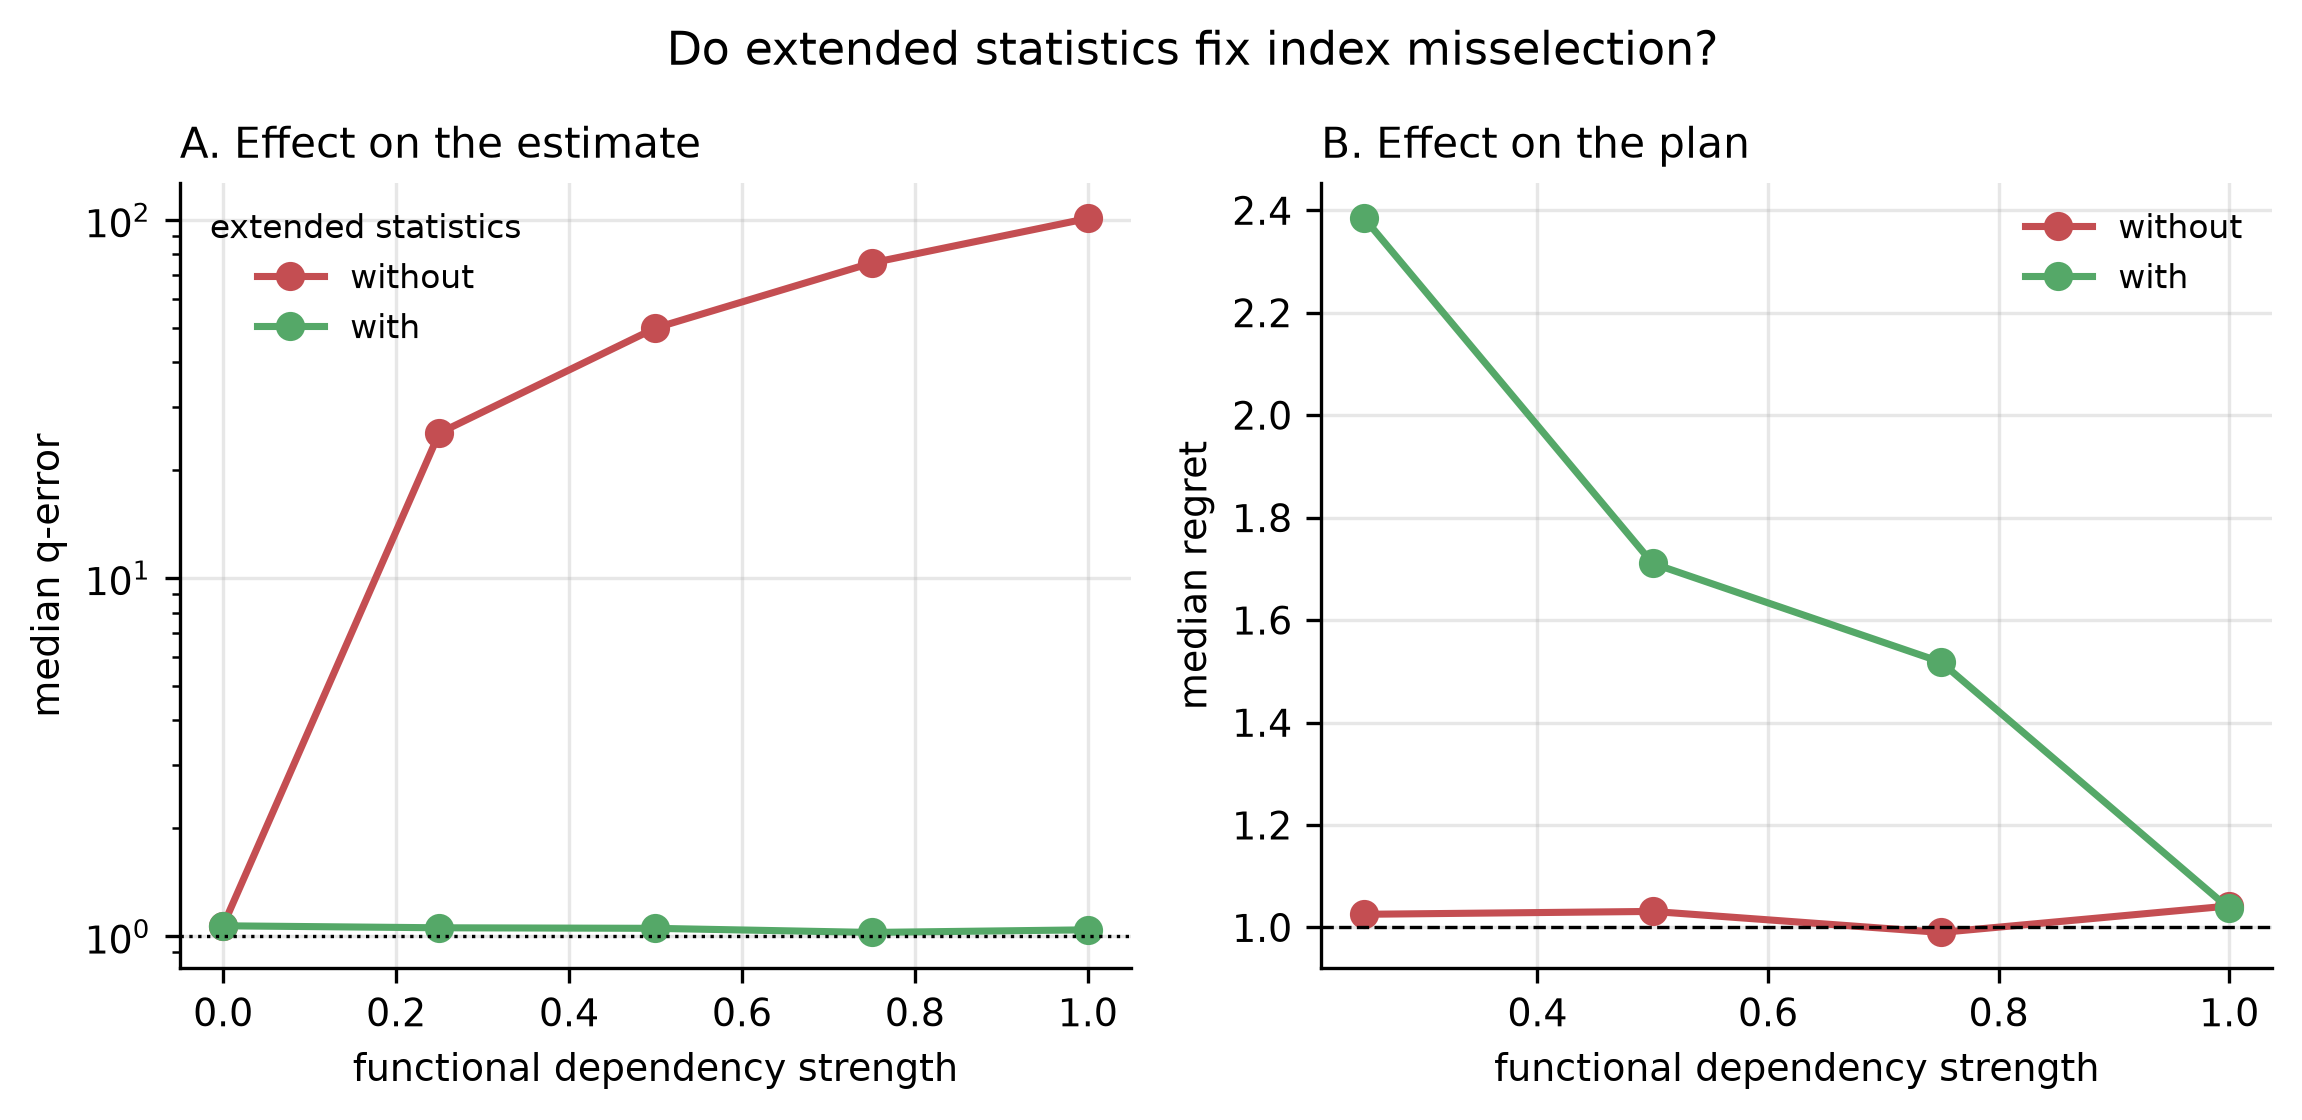
\includegraphics[width=0.95\linewidth]{figures/fig4_extended_statistics.png}
    \caption{Extended statistics against functional dependency
    strength. Panel A: the estimate improves by up to two orders of
    magnitude. Panel B: the resulting plan gets worse. Improving the
    estimate and improving the plan are separable outcomes.}
    \label{fig:extstats}
\end{figure}

\textbf{Mechanism.} The plans show the cause directly. Without extended
statistics the planner uses the composite index on \texttt{(a, b)} in a
single index scan. With them it switches to a \texttt{BitmapAnd} of two
single-column indexes. Both fetch the identical 7{,}317 heap blocks,
but the \texttt{BitmapAnd} performs two index scans plus a bitmap
intersection instead of one scan. The reason for the switch is visible
in the node estimates:

\begin{lstlisting}[caption={Node row estimates with extended statistics
present. The correction reaches the upper node but not the
\texttt{BitmapAnd} beneath it.}, label={lst:bitmapand}]
Bitmap Heap Scan  ... rows=10367     <- extended statistics applied
  -> BitmapAnd    ... rows=107       <- independence assumption, NOT corrected
\end{lstlisting}

Since $10367 \times 10367 / 10^6 \approx 107$, the \texttt{BitmapAnd}
node is still multiplying per-column selectivities under the
independence assumption that extended statistics exist to replace. The
planner therefore prices the \texttt{BitmapAnd} at 635 using the
\emph{uncorrected} figure and the composite path at 13{,}558 using the
\emph{corrected} one, a 21-fold gap, and selects the plan that is in
fact slower. The correction is applied inconsistently across path
types.

\subsection{RQ4b: Lowering \texttt{random\_page\_cost}}
The default \texttt{random\_page\_cost} of 4.0 assumes a random page
fetch costs four times a sequential one, a spinning-disk assumption.
Community guidance recommends lowering it on SSD storage. Measured
across the whole query set, that advice is wrong in this environment
(\Cref{tab:rpc}, \Cref{fig:rpc}).

\begin{table}[htbp]
    \centering
    \caption{Total execution time over the full query set at each
    \texttt{random\_page\_cost}, conventional index set. The default is
    within 6\% of optimal.}
    \label{tab:rpc}
    \small
    \begin{tabular}{@{}lrr@{}}
        \toprule
        \texttt{random\_page\_cost} & \textbf{Total time (ms)} & \textbf{Versus best} \\
        \midrule
        1.0            & 2{,}306 & \textbf{2.3$\times$ worse} \\
        1.1            & 1{,}954 & 1.9$\times$ worse \\
        1.2            & 1{,}942 & 1.9$\times$ worse \\
        \textbf{1.5}   & \textbf{1{,}006} & best \\
        2.0            & 1{,}053 & 1.0$\times$ \\
        3.0            & 1{,}053 & 1.0$\times$ \\
        \textbf{4.0} (default) & \textbf{1{,}068} & 1.06$\times$ \\
        \bottomrule
    \end{tabular}
\end{table}

\begin{figure}[htbp]
    \centering
    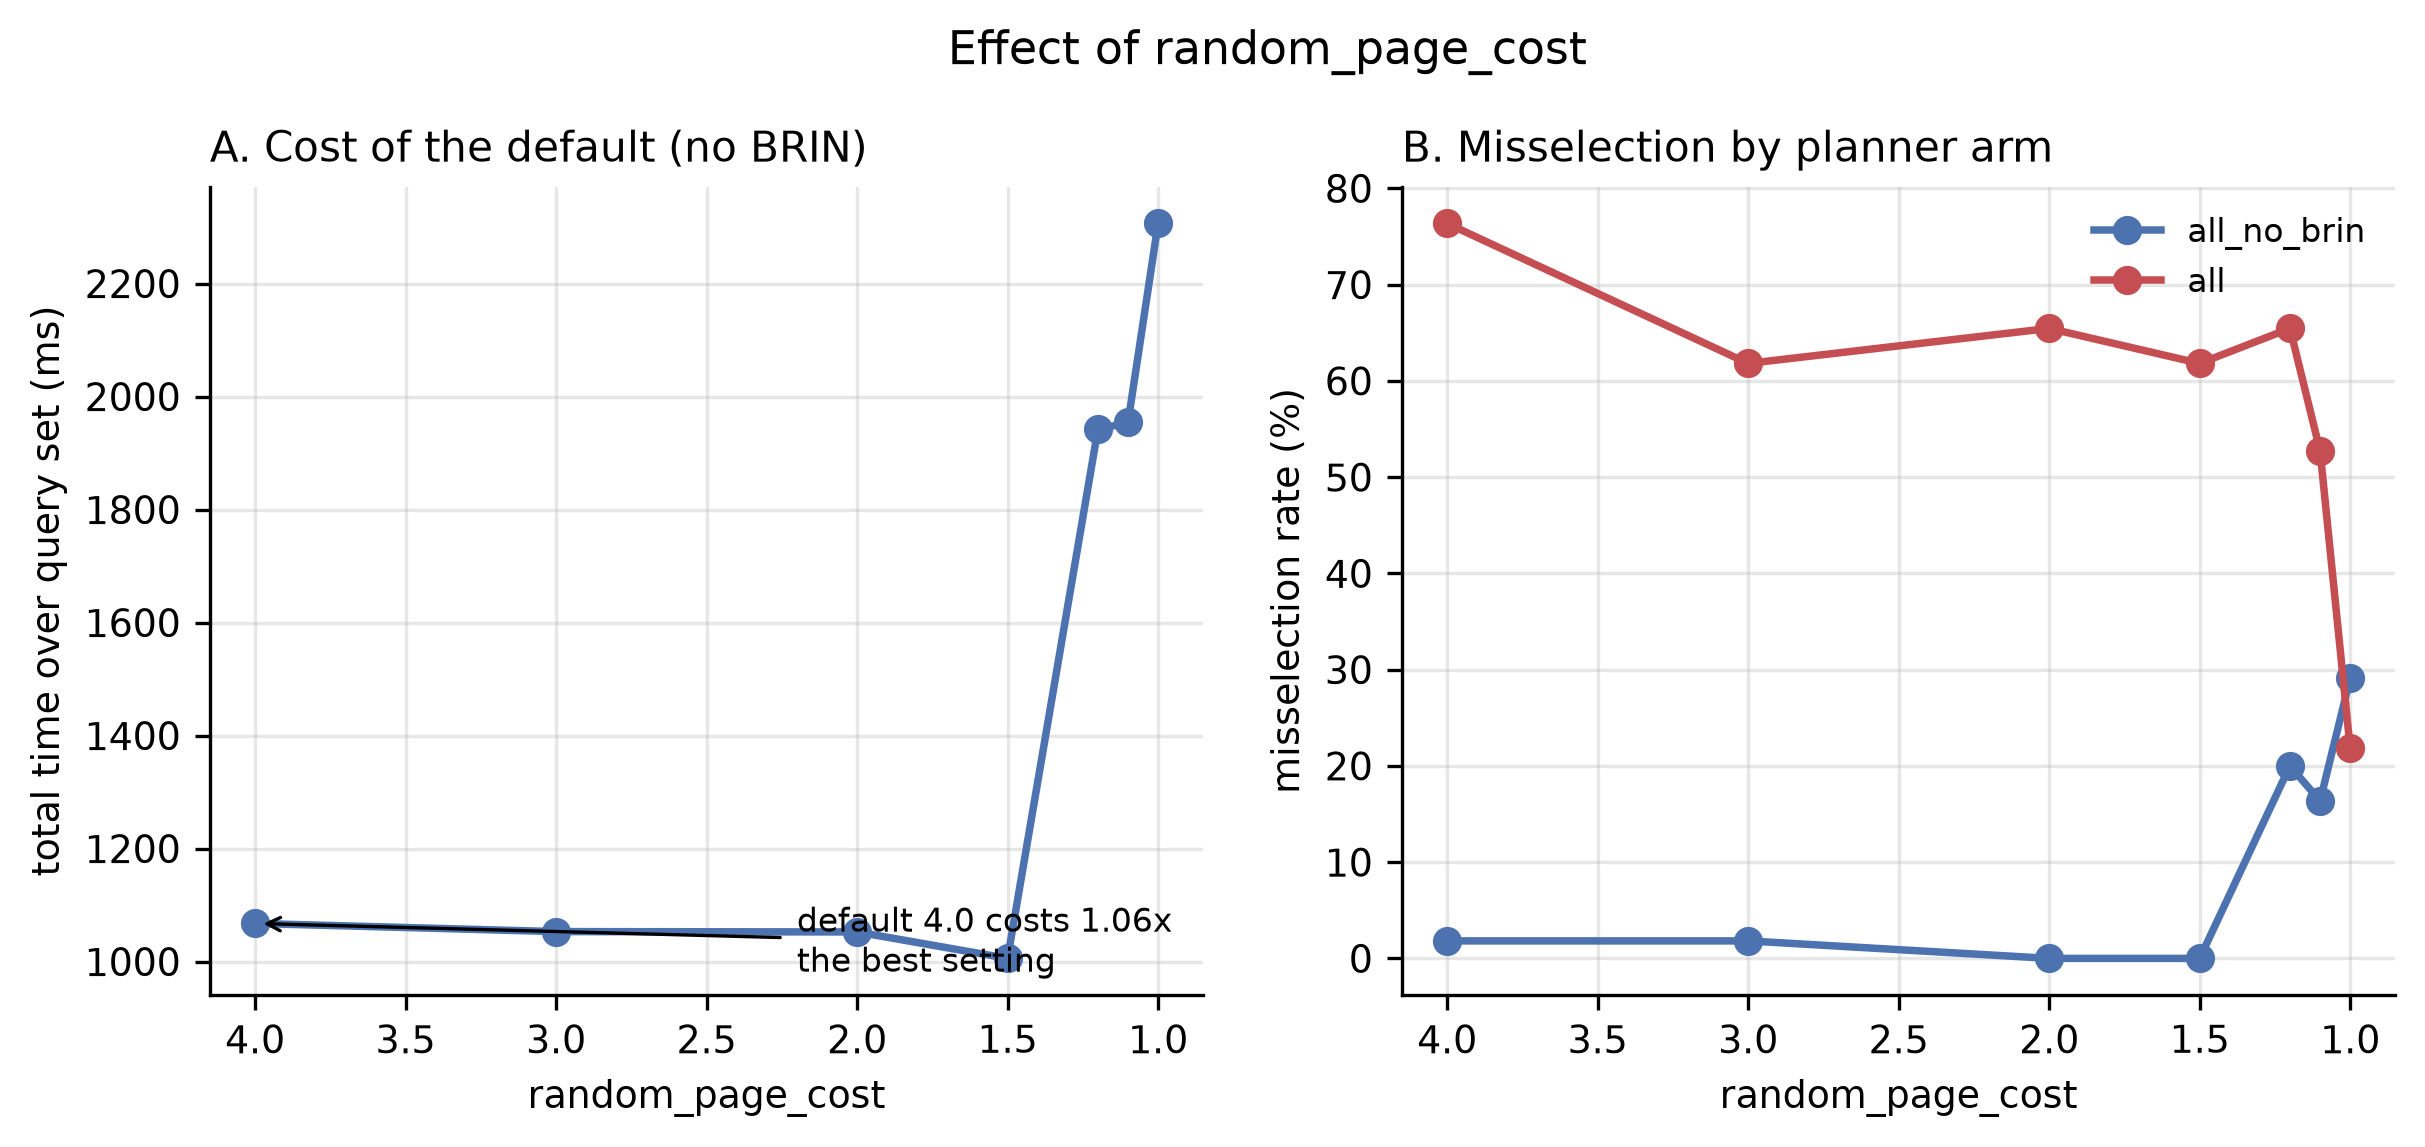
\includegraphics[width=0.95\linewidth]{figures/fig6_random_page_cost.png}
    \caption{Effect of \texttt{random\_page\_cost}. Panel A: total
    query-set time; lowering the setting below 1.5 degrades the
    workload. Panel B: misselection rate by index configuration.}
    \label{fig:rpc}
\end{figure}

The access-path counts explain why. At \texttt{random\_page\_cost = 1.0}
the planner abandons bitmap scans entirely in favour of plain index
scans, 136 index scans and zero bitmap scans, which is the wrong choice
for higher-selectivity predicates.

A single-query measurement early in this study suggested the default
cost 24 times (Appendix~\ref{app:plans}, \Cref{tab:rpcsingle}). That
observation was real but unrepresentative, and the workload-level sweep
supersedes it. It is retained deliberately as a caution against tuning
from individual queries.

\subsection{RQ2 and RQ4c: A Co-located BRIN Index}
BRIN indexes are small and cheap to build, so adding one is often
treated as harmless. It is not, while the table is buffer-pool resident
(\Cref{tab:brin}, \Cref{fig:brin}).

\begin{table}[htbp]
    \centering
    \caption{Effect of adding a BRIN index alongside an existing
    B-tree on the same column.}
    \label{tab:brin}
    \small
    \begin{tabular}{@{}lrrrr@{}}
        \toprule
        \textbf{Scale} & \textbf{With BRIN} & \textbf{Without BRIN} & \textbf{Median $R$} & \textbf{Max $R$} \\
        \midrule
        \textbf{1M}  & \textbf{73.3\%} & 2.3\%  & 2.06 vs 1.01 & \textbf{18.78} \\
        10M          & 30.1\%          & 32.3\% & 1.04 vs 1.04 & 2.63 \\
        \bottomrule
    \end{tabular}
\end{table}

\begin{figure}[htbp]
    \centering
    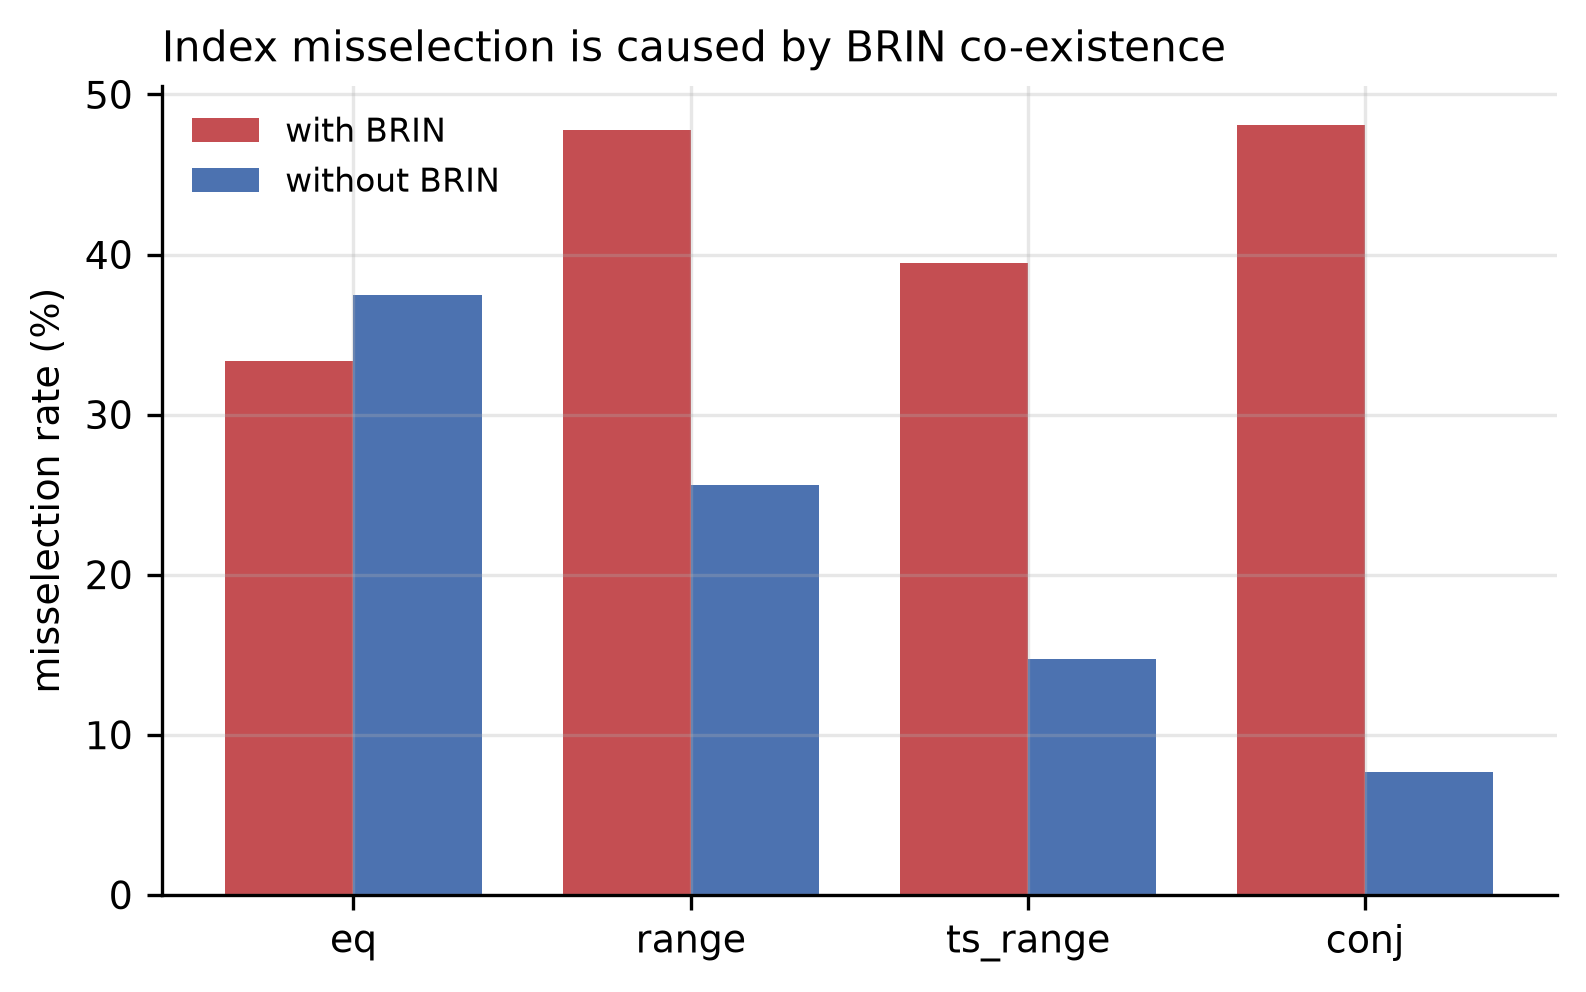
\includegraphics[width=0.68\linewidth]{figures/fig0_brin_effect.png}
    \caption{Misselection rate by query family with and without a BRIN
    index in the index set, 1M rows. The conjunctive family is the
    control: no BRIN index touches those columns, and correspondingly
    there is no effect.}
    \label{fig:brin}
\end{figure}

At one million rows, adding a BRIN index alongside an existing B-tree
raises misselection from 2.3\% to 73.3\%. In controlled diagnostics
with statistics held byte-identical, individual queries degraded by up
to \textbf{194 times}, from 0.34\,ms to 65.95\,ms.

\textbf{Mechanism.} With both indexes present and a bitmap plan forced,
the planner selected BRIN in \textbf{16 of 16 cases}, and in ten of
those the B-tree bitmap path was cheaper \emph{by the planner's own
cost model}, once by a factor of nine. A cost-based optimiser does not
knowingly select a path it prices as nine times more expensive, which
indicates the B-tree bitmap path is discarded during path generation
rather than rejected on cost. This is an inference from cost arithmetic
and has not been confirmed against PostgreSQL's source.

The cost of the chosen plan is visible in its execution:
\texttt{Heap Blocks: lossy=14304} with
\texttt{Rows Removed by Index Recheck: 990000}. BRIN reads essentially
the whole table and discards 99\% of what it reads.

\Cref{fig:brincorr} shows how each index type responds to the physical
correlation BRIN depends on.

\begin{figure}[htbp]
    \centering
    
\includegraphics[width=0.68\linewidth]{figures/fig5_brin_correlation.png}
    \caption{Execution time against physical correlation of the indexed
    column for each index configuration. BRIN becomes viable only as
    correlation approaches 1.}
    \label{fig:brincorr}
\end{figure}

\subsection{Locating the Boundary}
\label{sec:boundary}
Comparing one million against ten million rows shows the penalty
present at the smaller scale and absent at the larger, but two points
cannot distinguish a gradual decay from a sharp transition. We
therefore repeated the measurement at five intermediate scales, using
the \texttt{phys} datasets so the comparison is like for like
(\Cref{tab:transition}, \Cref{fig:transition}).

\begin{table}[htbp]
    \centering
    \caption{The BRIN penalty across table size. Two quantities move
    independently: how \emph{often} the planner errs, and how
    \emph{badly} it errs in the worst case.}
    \label{tab:transition}
    \small
    \begin{tabular}{@{}rrrrrrr@{}}
        \toprule
        \textbf{Million} & \textbf{Heap} & \textbf{Blocks read} & \multicolumn{2}{c}{\textbf{Misselection \%}} & \multicolumn{2}{c}{\textbf{Max regret}} \\
        \cmidrule(lr){4-5}\cmidrule(lr){6-7}
        \textbf{rows} & \textbf{(MB)} & \textbf{outside pool} & with BRIN & without & with BRIN & without \\
        \midrule
        1.00  & 111.8   & 0       & \textbf{71.4} & 0.0  & 18.78 & 1.06 \\
        1.25  & 139.8   & 0       & 37.9 & 34.5 & \textbf{38.81} & 1.67 \\
        1.50  & 167.8   & 0       & 31.0 & 17.2 & \textbf{40.32} & 1.76 \\
        2.00  & 223.2   & 0       & 25.8 & 12.9 & \textbf{38.34} & 1.77 \\
        3.00  & 335.2   & 0       & 30.3 & 12.1 & \textbf{41.51} & 1.67 \\
        5.00  & 558.2   & 1{,}902 & 36.4 & 30.3 & 6.98 & 1.81 \\
        10.00 & 1{,}116.2 & 89{,}081 & 38.2 & 44.4 & 1.92 & 3.70 \\
        \bottomrule
    \end{tabular}
\end{table}

\begin{figure}[htbp]
    \centering
    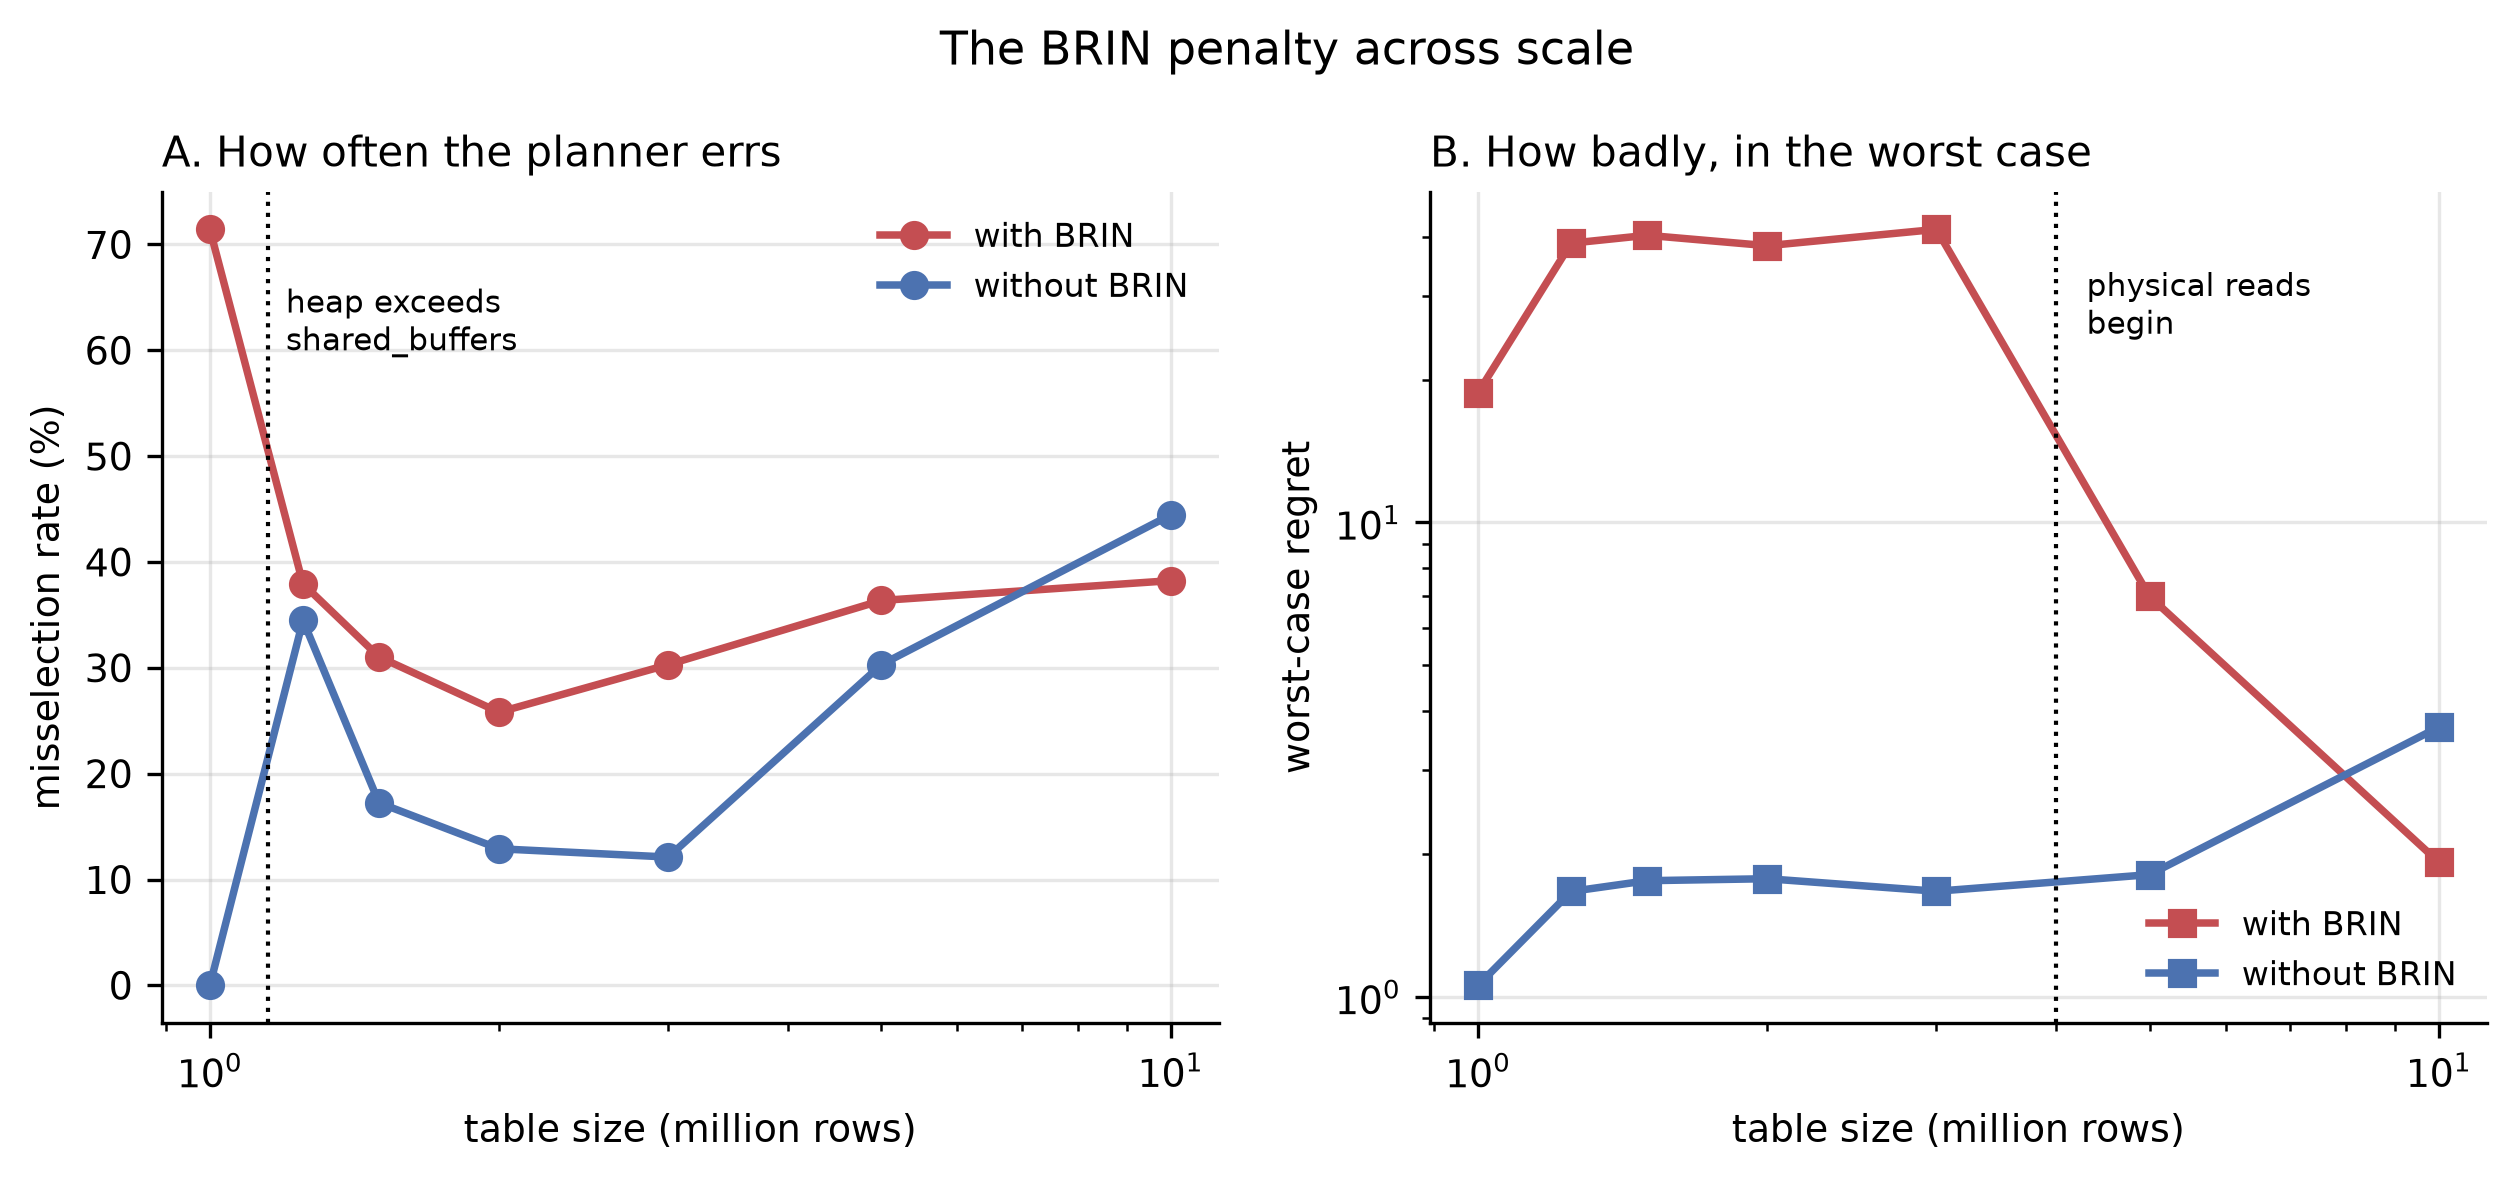
\includegraphics[width=0.95\linewidth]{figures/fig7_scale_transition.png}
    \caption{The BRIN penalty across scale. Panel A: how often the
    planner errs. Panel B: worst-case regret. The two collapse at
    different table sizes, near two different system boundaries.}
    \label{fig:transition}
\end{figure}

The transition is sharp, and there are \emph{two} of them.

\textbf{Frequency collapses at the buffer pool boundary.} The gap in
misselection rate falls from 71.4 percentage points at one million rows
to 3.4 at 1.25 million. That is precisely where the heap crosses
\texttt{shared\_buffers}: 111.8\,MB against the 128\,MB pool at one
million rows, 139.8\,MB at 1.25 million. Note what drives the collapse:
the with-BRIN configuration improves from 71.4\% to 37.9\%, but the
conventional configuration \emph{degrades} from 0.0\% to 34.5\%. The
gap closes largely because the baseline gets worse, not because BRIN
gets better.

\textbf{Severity collapses much later, and first gets worse.}
Worst-case regret with BRIN does not decline past the buffer pool
boundary. It roughly doubles, from 18.78 at one million rows to 38.81
at 1.25 million, and stays near 40 through three million. It falls only
at five million (6.98) and ten million (1.92). That later collapse
coincides with the onset of physical reads: blocks fetched from outside
the buffer pool are zero up to three million rows, 1{,}902 at five
million and 89{,}081 at ten million.

This corrects a conclusion that two-point comparison would have
supported. The BRIN penalty does not simply vanish with scale. Its
\emph{frequency} falls once the table stops fitting in the buffer pool,
while its \emph{worst case} intensifies over the next several-fold
increase in table size and subsides only once queries begin paying real
I/O. A practitioner whose table is two or three times the buffer pool
faces the most severe individual regressions measured anywhere in this
study.

We do not claim a verified causal mechanism for either transition. What
is established is that each coincides with a specific, measurable
system boundary, and that the two boundaries are different.

\subsection{Incidental Finding: Hash Index Build Cost Under Skew}
Hash index build time proved highly sensitive to value skew
(\Cref{tab:hashbuild}), a 185-fold blowup from uniform to heavily
skewed data while a B-tree on the same column is unaffected. Zipfian
values collide into few hash buckets, producing long overflow chains,
and PostgreSQL does not parallelise hash builds as it does B-tree
builds.

\begin{table}[htbp]
    \centering
    \caption{Index build time at 10M rows by value skew.}
    \label{tab:hashbuild}
    \small
    \begin{tabular}{@{}lrrr@{}}
        \toprule
        \textbf{Dataset} & \texttt{zipf\_s} & \textbf{Hash build} & \textbf{B-tree build} \\
        \midrule
        baseline & 0.0 & 11.6 s & 3.2 s \\
        skew05   & 0.5 & 16.7 s & 2.3 s \\
        skew10   & 1.0 & 187.7 s & 2.5 s \\
        \textbf{skew15} & \textbf{1.5} & \textbf{2{,}152.9 s} & 2.3 s \\
        \bottomrule
    \end{tabular}
\end{table}

\subsection{Analysis and Interpretation}
\Cref{fig:regret} places the results in context by plotting regret
against true selectivity. Misselection concentrates in the one to ten
percent selectivity band, which is exactly where the cost of an index
scan and a sequential scan converge and where small cost-model errors
therefore flip the decision.

\begin{figure}[htbp]
    \centering
    
\includegraphics[width=0.68\linewidth]{figures/fig2_regret_by_selectivity.png}
    \caption{Access-path regret against true selectivity, by query
    family. The dashed line at $R = 1$ marks optimal choice.}
    \label{fig:regret}
\end{figure}

The mechanism is consistent across all three failures. A bitmap heap
scan's cost is dominated by the number of heap pages it expects to
fetch, priced at \texttt{random\_page\_cost}. Any error in that
estimate, whether from a lossy BRIN bitmap, an uncorrected
\texttt{BitmapAnd} node, or a miscalibrated page-cost constant, moves
the crossover point between index and sequential access. Because the
true execution times on either side of that crossover differ sharply,
a small pricing error produces a large runtime penalty.

%=====================================================================
\section{Discussion}
\label{sec:discussion}
%=====================================================================

\subsection{Key Insights}
The three practices fail for the same underlying reason: each is
justified by reasoning about a single quantity, while plan quality
depends on several.

Extended statistics optimise \textbf{estimate accuracy}, and a more
accurate estimate improves the plan only if applied consistently
wherever the plan is costed. It is not.

Lowering \texttt{random\_page\_cost} optimises for \textbf{storage
latency}, and it is true that random access on SSD is cheaper than the
default assumes. But the same constant governs the choice between
bitmap and plain index scans, so pushing it too low wins on one axis
and loses on another.

Adding a BRIN index optimises for \textbf{index size and build cost},
both of which genuinely favour BRIN. But index availability also
changes which paths the planner generates, and a cheap index that
captures the bitmap path can exclude a better one.

In each case the advice is correct about the quantity it names and
wrong about the outcome, because the outcome depends on more than that
quantity. This is a general caution about mechanism-based tuning advice
that has not been validated at the workload level.

\subsection{Connection to Course Concepts}
The work applies several core topics from the course directly.
\emph{Indexing}: the trade-off between B-tree, hash and BRIN structures
is measured rather than asserted, including the dependence of BRIN on
physical clustering and of hash on value distribution.
\emph{Query processing and optimisation}: the System R cost-based
framework~\cite{selinger1979access} is exercised at its weakest point,
the transition between access paths, and the propagation of selectivity
estimates through a plan tree is observed directly in
\Cref{lst:bitmapand}. \emph{Storage management}: the buffer pool
residency boundary in \Cref{sec:results} is precisely the distinction
between logical reads served from \texttt{shared\_buffers} and physical
reads issued beyond it, and it turns out to determine whether an entire
finding holds.

\subsection{Recommendations for Practitioners}
\begin{enumerate}[nosep]
    \item Do not add extended statistics reflexively. Verify that the
      \emph{plan} improved, not merely the estimate. The two are
      separable.
    \item Do not lower \texttt{random\_page\_cost} below approximately
      1.5 without measuring. The default was within 6\% of optimal here.
    \item Treat a BRIN index alongside a B-tree on the same column as a
      risk to be measured, particularly where the table fits in the
      buffer pool.
    \item Do not assume hash index creation is cheap on skewed columns.
\end{enumerate}

\subsection{Limitations and Threats to Validity}

\textbf{Internal validity.} Regret is a lower bound, since the
denominator is the fastest measured configuration rather than a proven
optimum. Values slightly below 1.0 occur because the planner can
combine indexes in ways no single restricted configuration can. The 1.2
misselection threshold is a judgement call.

\textbf{Construct validity.} The path-suppression mechanism in
\Cref{sec:results} is inferred from cost arithmetic, not confirmed
against PostgreSQL's source code. The extended statistics result
requires a redundant index set, a composite index plus both
single-column indexes, which is common in practice but not universal.

\textbf{External validity.} One DBMS, one version, one hardware
configuration. All measurements are warm-cache; reliably evicting the
operating system page cache is not portable across platforms, so
cold-storage behaviour is out of scope rather than approximated.
With 23.8\,GB of RAM the page cache retains the data even at ten
million rows, so the larger scale tests leaving the \emph{buffer pool},
not leaving memory. Single-table access paths only.

%=====================================================================
\section{Conclusion and Recommendations}
\label{sec:conclusion}
%=====================================================================
PostgreSQL 17's access-path selection is close to optimal under a
conventional index set, choosing the best available plan for 97.7\% of
the queries measured. Where it fails, cardinality misestimation is not
the cause: 98.2\% of misselected queries had accurate row estimates.
This contrasts with the established result for join
ordering~\cite{leis2015good} and suggests the access-path decision has
a different failure profile.

The failures instead trace to the cost model and to path generation,
and are triggered by three practices intended to help. Extended
statistics improve estimates by up to 108 times and slow queries by up
to 2.7 times, because the correction is not propagated to the
\texttt{BitmapAnd} node. Lowering \texttt{random\_page\_cost} on SSD,
contrary to common advice, costs a factor of 2.3 in this workload, the
default being within 6\% of optimal. A co-located BRIN index raises
misselection from 2.3\% to 73.3\% and can slow individual queries by
194 times while the table is buffer-pool resident.

The boundaries are as much a part of that last result as the effect
itself, and measuring them changed what we could claim. A two-point
comparison, one million rows against ten million, would have supported
the conclusion that the penalty simply vanishes with scale. Five
intermediate scales show otherwise: its frequency collapses once the
heap exceeds \texttt{shared\_buffers}, but its worst case roughly
doubles at that same point and subsides only once queries begin paying
physical I/O, several-fold further out. The most severe individual
regressions in this entire study occur at two to three times the buffer
pool size, not at the smallest scale.

That is the general lesson. A tuning recommendation is not right or
wrong in isolation; it is right or wrong under conditions, and those
conditions are measurable. Reporting an effect without its boundary
invites practitioners to apply it where it does not hold, or to dismiss
it where it does.

\textbf{Future work.} Three directions would strengthen these findings:
confirming the path-suppression mechanism against PostgreSQL's source
code; repeating the study on a second DBMS to test whether the results
are PostgreSQL-specific; and extending to cold-cache conditions on
hardware where page cache eviction is controllable, which would
separate buffer pool residency from operating system page cache
residency, a distinction the present hardware cannot make.

%---------------------------------------------------------------------
\newpage
\printbibliography[heading=bibnumbered, title={References}]

%---------------------------------------------------------------------
% APPENDICES
%---------------------------------------------------------------------
\newpage
\appendix

\section{Query Execution Plans}
\label{app:plans}

All plans below are unmodified \texttt{EXPLAIN} output captured during
the study. The script producing each is named, so any can be
regenerated from the artifact~\cite{artifact2026}.

\subsection{The BRIN Effect With Statistics Held Constant}
Source: \texttt{diagnose\_brin.py}. 1M rows,
\texttt{physical\_corr = 0.5}. Both indexes exist on \texttt{ts}.
\texttt{ANALYZE} was run once and never again, so both plans below come
from byte-identical statistics. The generator's realised rank
correlation was 0.4984 and PostgreSQL's own \texttt{pg\_stats} estimate
0.49863, confirming the intended clustering.

\begin{lstlisting}[caption={Plan chosen with both indexes available.}]
Bitmap Heap Scan on t_brindiag  (cost=14.56..14858.18 rows=9705) (actual rows=10000)
  Recheck Cond: ((ts >= 1655753994) AND (ts <= 1657336369))
  Rows Removed by Index Recheck: 990000
  Heap Blocks: lossy=14304
  Buffers: shared hit=2696 read=11616
  ->  Bitmap Index Scan on ix_brindiag_brin_ts  (cost=0.00..12.13 rows=35975)
Execution Time: 132.691 ms
\end{lstlisting}

\begin{lstlisting}[caption={Same query, same statistics, BRIN index removed.}]
Bitmap Heap Scan on t_brindiag  (cost=215.87..14045.79 rows=10092) (actual rows=10000)
  Recheck Cond: ((ts >= 1655753994) AND (ts <= 1657336369))
  Heap Blocks: exact=4293
  Buffers: shared hit=4293 read=30
  ->  Bitmap Index Scan on ix_brindiag_btree_ts  (cost=0.00..213.35 rows=10092)
Execution Time: 3.416 ms
\end{lstlisting}

Note \texttt{lossy=14304} against \texttt{exact=4293}, and 132.691\,ms
against 3.416\,ms. The planner priced the chosen plan at 14{,}858 and
the unchosen one at 14{,}046, so the plan it did not use was the
cheaper one by its own model.

\subsection{Path Suppression Across the Correlation Range}
Source: \texttt{diagnose\_suppression.py}. Bitmap plans forced by
disabling all other access methods, statistics held constant within
each row.

\begin{table}[htbp]
    \centering
    \caption{BRIN was selected in 16 of 16 cases. In ten the B-tree
    bitmap path was cheaper by the planner's own cost model.}
    \label{tab:suppression}
    \small
    \begin{tabular}{@{}llrrrr@{}}
        \toprule
        \textbf{Corr.} & \textbf{Query} & \textbf{BRIN cost} & \textbf{BRIN ms} & \textbf{B-tree cost} & \textbf{B-tree ms} \\
        \midrule
        0.0  & 0.1\% range & 29{,}320 & 65.95 & 3{,}166  & \textbf{0.34} \\
        0.0  & 1\% range   & 29{,}322 & 66.73 & 13{,}857 & 5.14 \\
        0.0  & 5\% range   & 29{,}332 & 69.50 & 16{,}111 & 12.87 \\
        0.5  & 0.1\% range & 15{,}338 & 66.33 & 3{,}174  & \textbf{0.21} \\
        0.5  & 1\% range   & 14{,}852 & 63.90 & 13{,}848 & 2.76 \\
        0.95 & 0.1\% range & 13{,}511 & 62.07 & 3{,}294  & \textbf{0.09} \\
        0.95 & 1\% range   & 15{,}365 & 66.45 & 14{,}201 & 0.76 \\
        1.0  & 0.1\% range & 13{,}286 & 0.55  & 2{,}903  & 0.07 \\
        \bottomrule
    \end{tabular}
\end{table}

The largest observed penalty is the 0.95 correlation, 0.1\% range case:
62.07\,ms against 0.09\,ms, a factor of 690.

\subsection{Extended Statistics Change the Plan for the Worse}
Source: \texttt{diagnose\_extstats.py}. 1M rows,
\texttt{dep\_strength = 1.0}, query
\texttt{SELECT * FROM t\_ext WHERE a = 57 AND b = 84}, true rows
10{,}216. Identical table, data, indexes and session; only the
extended statistics object is added.

\begin{lstlisting}[caption={Without extended statistics. Median of 15 runs: 4.059 ms (stdev 0.473).}]
Bitmap Heap Scan on t_ext  (cost=5.38..356.28 rows=93) (actual rows=10216)
  Heap Blocks: exact=7317
  ->  Bitmap Index Scan on ix_ext_ab  (cost=0.00..5.35 rows=93)
        Index Cond: ((a = 57) AND (b = 84))
\end{lstlisting}

\begin{lstlisting}[caption={With extended statistics. Median of 15 runs: 5.171 ms (stdev 0.261).}]
Bitmap Heap Scan on t_ext  (cost=219.84..559.77 rows=9467) (actual rows=10216)
  Heap Blocks: exact=7317
  ->  BitmapAnd  (cost=219.84..219.84 rows=90)
        ->  Bitmap Index Scan on ix_ext_b  (cost=0.00..107.43 rows=9467)
        ->  Bitmap Index Scan on ix_ext_a  (cost=0.00..107.43 rows=9467)
\end{lstlisting}

The two timing distributions do not overlap, so this is not
measurement noise. Both plans fetch the identical 7{,}317 heap blocks.

\subsection{Confirming the Planner Acts Rationally on Its Own Model}
Source: \texttt{diagnose\_composite.py}. With correct estimates the
planner prices the composite path at 13{,}558 and the
\texttt{BitmapAnd} at 635, a 21-fold gap, while the composite path is
in fact the faster of the two (\Cref{tab:composite}). Without extended
statistics the same composite path is priced at 392.80 and runs in
4.155\,ms: the \emph{correct} estimate makes the plan appear 34 times
more expensive while running at the same speed.

\begin{table}[htbp]
    \centering
    \caption{Plan cost and measured time by available index set,
    extended statistics present.}
    \label{tab:composite}
    \small
    \begin{tabular}{@{}llrr@{}}
        \toprule
        \textbf{Indexes available} & \textbf{Plan chosen} & \textbf{Total cost} & \textbf{Median ms} \\
        \midrule
        all three       & \texttt{BitmapAnd} of $a$, $b$ & 635.63     & 4.794 \\
        composite only  & composite $(a,b)$              & 13{,}558.73 & \textbf{4.030} \\
        separate only   & \texttt{BitmapAnd}             & 643.90     & 5.357 \\
        \bottomrule
    \end{tabular}
\end{table}

\subsection{Cost Model Sensitivity on a Single Query}
Source: \texttt{diagnose.py}. Same query, same data, identical row
estimate (10{,}662) throughout; only \texttt{random\_page\_cost}
changes.

\begin{table}[htbp]
    \centering
    \caption{Single-query sensitivity to \texttt{random\_page\_cost}.
    Taken alone this suggests the default is catastrophic; measured
    across the whole query set (\Cref{tab:rpc}) it is within 6\% of
    optimal.}
    \label{tab:rpcsingle}
    \small
    \begin{tabular}{@{}lrr@{}}
        \toprule
        \texttt{random\_page\_cost} & \textbf{Plan chosen} & \textbf{Median ms} \\
        \midrule
        4.0 (default) & sequential scan     & 49.14 \\
        2.0           & B-tree index scan   & \textbf{2.08} \\
        1.5           & B-tree index scan   & 2.33 \\
        1.1           & B-tree index scan   & 2.49 \\
        1.0           & B-tree index scan   & 2.25 \\
        \bottomrule
    \end{tabular}
\end{table}

\subsection{Buffer Pool Residency}
Median buffer counters for range queries on the physically clustered
column, full index set. \texttt{shared\_read} counts blocks fetched
from outside the buffer pool: zero at one million rows confirms full
residency, 89{,}081 at ten million confirms the working set has left
the pool. This is the independent evidence that the two scales are
genuinely different regimes.

\begin{table}[htbp]
    \centering
    \caption{Buffer statistics by scale.}
    \label{tab:buffers}
    \small
    \begin{tabular}{@{}lrr@{}}
        \toprule
        \textbf{Scale} & \texttt{shared\_hit} & \texttt{shared\_read} \\
        \midrule
        1{,}000{,}000 rows  & 13{,}194 & \textbf{0} \\
        10{,}000{,}000 rows & 11{,}314 & \textbf{89{,}081} \\
        \bottomrule
    \end{tabular}
\end{table}

\section{Reproducibility}
All code, raw measurements, figures and an executable analysis notebook
are published~\cite{artifact2026}. No dataset is shipped: all data is
generated from a fixed seed, so the corpus is byte-for-byte identical
on any machine.

\begin{lstlisting}[caption={Complete reproduction sequence.}]
pip install -r research/requirements.txt
psql -c "CREATE TABLESPACE ts_dtms LOCATION '/path/with/space';"

python research/tests/test_generator.py         # validate the generator
python research/tests/test_range_targeting.py   # validate query construction
python research/run_experiment.py --rows 1000000
python research/run_experiment.py --rows 10000000
python research/run_rpc_sweep.py
python research/analyze.py                      # regenerates every figure
\end{lstlisting}

Runs are resumable at the granularity of a single measurement: every
result is appended to disk as it is taken, and the resume key is
(dataset, index configuration, query, extended-statistics state). This
was exercised twice during the study, once by a stopped process and
once by a power failure; both times the loss was a single in-flight
query.

Each measurement record retains all individual runs, not only the
median, so the variance claims in this report can be checked
independently.

\section{Individual Contribution Statement}
\begin{table}[htbp]
    \centering
    \caption{Individual contributions.}
    \label{tab:contrib}
    \small
    \begin{tabular}{@{}lp{9cm}@{}}
        \toprule
        \textbf{Member} & \textbf{Contribution} \\
        \midrule
        Md. Imtiaj Alam Sajin & Experimental design; benchmark implementation;
        data generation and validation; measurement infrastructure;
        diagnostics; analysis; all sections of this report. \\
        \bottomrule
    \end{tabular}
\end{table}

\end{document}
